\documentclass[letterpaper]{article} % DO NOT CHANGE THIS
\usepackage[submission]{aaai2027}  % DO NOT CHANGE THIS
\usepackage[hyphens]{url}  % DO NOT CHANGE THIS
\usepackage{graphicx} % DO NOT CHANGE THIS
\urlstyle{rm} % DO NOT CHANGE THIS
\def\UrlFont{\rm}  % DO NOT CHANGE THIS
\usepackage{natbib}  % DO NOT CHANGE THIS
\usepackage{caption} % DO NOT CHANGE THIS
\frenchspacing  % DO NOT CHANGE THIS
\usepackage{amsmath}
\usepackage{amssymb}
\usepackage{amsthm}
\usepackage{booktabs}

\pdfinfo{
/TemplateVersion (2027.1)
}

\setcounter{secnumdepth}{1}
\newtheorem{theorem}{Theorem}
\newcommand{\sg}{\mathrm{sg}}
\newcommand{\softmax}{\mathrm{softmax}}

\title{Supplementary Material:\\
A Differentiable Atari VCS: A Complex, Fully Known\\
Ground Truth for Explainable AI}
\author{Anonymous Submission}
\affiliations{}

\begin{document}
\maketitle

This supplement gives the full proofs of the two theorems stated in the main
paper, together with the implementation-effort plot referenced in the Results.
It is self-contained: we first restate the soft/hard formulation, then prove the
forward-equivalence and temperature-limit results, and finally show the effort
timeline.

\section{Setup and Notation}

The differentiable emulator runs one of two transition maps over the full VCS
state $x=(\text{registers},\text{RAM},\text{RIOT},\text{TIA},\text{frame
buffer})$: the bit-exact \emph{hard} map $\Phi_{\mathrm{H}}$ and the
differentiable \emph{soft} map $\Phi_{\mathrm{S}}$. Both are the per-opcode
handler selected by the byte at the program counter ($\mathrm{pc}$). Four
primitives appear in the handlers.

\emph{One-hot reads.} A ROM or RAM read at integer address $a$ is the dot
product
\begin{equation}
\mathrm{peek}(r,a)=\mathbf{1}_a^{\top}r=\textstyle\sum_i[\![i=a]\!]\,r_i=r_a .
\label{eq:s-peek}
\end{equation}

\emph{Softmax dispatch.} With a score vector (logits) $\ell\in\mathbb{R}^{K}$
over the $K=256$ opcodes, temperature $T>0$, and softmax weights
$w=\softmax(\ell/T)$, the relaxed dispatch output over candidate handler rows
$V$ is
\begin{equation}
\mathrm{select}(\ell,V;T)=w^{\top}V,\qquad
w_k=\frac{e^{\ell_k/T}}{\sum_j e^{\ell_j/T}} .
\label{eq:s-select}
\end{equation}

\emph{Sigmoid branch.} For a relaxed status flag $f\in[0,1]$ written as a logit
$z=s(2f-1)$ (sign $s$ for branch-when-set/clear) and sharpness $\alpha$, the
gate and relaxed program counter are
\begin{equation}
g=\sigma(\alpha z),\qquad
\mathrm{pc}_{\mathrm{soft}}=(1-g)\,\mathrm{pc}_{\bar b}+g\,\mathrm{pc}_{b}.
\label{eq:s-branch}
\end{equation}

\emph{Straight-through estimator.} For a soft value with a matching hard value,
\begin{equation}
\mathrm{STE}(\text{soft},\text{hard})=\text{soft}+\sg(\text{hard}-\text{soft}),
\label{eq:s-ste}
\end{equation}
whose forward value is \textit{hard} and whose gradient is that of \text{soft}.

In the executed soft step, dispatch uses the saturated (hard) form of
\eqref{eq:s-select}, and the branch returns
$\mathrm{STE}(\mathrm{pc}_{\mathrm{soft}},\mathrm{pc}_{\mathrm{hard}})$;
\eqref{eq:s-select} and \eqref{eq:s-branch} in their relaxed form define the
``fully relaxed'' variant analysed in Theorem~2.

\paragraph{Assumption (DM, decision margins).} Along the executed trajectory of
length $N$, every discrete decision has a strictly positive margin: each
dispatch has a logit gap $\Delta=\ell_{k^\star}-\max_{k\ne k^\star}\ell_k\ge
\Delta_{\min}>0$, and each branch has a margin $m=|z|\ge m_{\min}>0$.

\section{Proofs}

\noindent\textbf{Theorem 1 (exact forward equivalence).} \emph{For every
reachable state $x$ and every finite $\alpha,T$, $\Phi_{\mathrm{S}}(x)=
\Phi_{\mathrm{H}}(x)$; hence $x^{\mathrm{S}}_t=x^{\mathrm{H}}_t$ for all $t\le N$.
The two modes differ only in the Jacobian.}

\begin{proof}
It suffices to show that, for each opcode, the soft and hard handlers produce
the same output value; the state is then carried forward identically. Each
handler is composed of four kinds of primitive.

\emph{(i) Memory reads.} A ROM or RAM read at integer address $a$ is the one-hot
dot product~\eqref{eq:s-peek}. Because $a$ is an integer index, $\mathbf{1}_a$
is exact and $\mathrm{peek}(r,a)=r_a$, identical to a hard array read.

\emph{(ii) Arithmetic.} Register, status-flag, binary-coded-decimal (BCD), and
RIOT-timer updates use the same integer and $\mathrm{round}$ operations as the
hard handlers; the soft path stores these quantities as float32 but computes
them with integer semantics, so their outputs are equal.

\emph{(iii) Dispatch.} The handler is chosen by a hard switch on the decoded
opcode byte, exactly as in hard mode; the softmax form~\eqref{eq:s-select} is
not used on the forward path.

\emph{(iv) Branch.} A conditional branch forms $\mathrm{pc}_{\mathrm{soft}}$
from~\eqref{eq:s-branch} but returns
$\mathrm{STE}(\mathrm{pc}_{\mathrm{soft}},\mathrm{pc}_{\mathrm{hard}})$
\eqref{eq:s-ste}. As $\sg$ is the identity on the forward pass, this equals
$\mathrm{pc}_{\mathrm{hard}}$ for every $\alpha$ and $T$.

Each primitive's forward output thus equals the hard handler's, so
$\Phi_{\mathrm{S}}(x)=\Phi_{\mathrm{H}}(x)$ for every reachable $x$; the hard
handlers are themselves validated bit-for-bit against \textsc{xitari} by the
conformance harnesses. By induction over the $N$ steps of a trajectory,
$x^{\mathrm{S}}_t=x^{\mathrm{H}}_t$ for all $t\le N$.

\emph{Bit-exactness.} float32 represents every integer in $[0,2^{24}]$ exactly,
and all VCS quantities lie in this range---data bytes are at most $255$,
addresses are $13$ bits, and per-frame cycle counts are a few tens of
thousands---so the float32 results are not merely close to the integer results
but identical.

\emph{Gradients.} The stop-gradient in~(iv) alters only the reverse-mode rule:
it sets $\partial\,\mathrm{STE}=\partial\,\mathrm{pc}_{\mathrm{soft}}$, the
derivative of the sigmoid-blended counter, which is generically nonzero where
the hard branch (a step function of the flag) has zero or undefined derivative;
likewise the read in~(i) has Jacobian $\mathbf{1}_a$ with respect to $r$. The
forward pass is unchanged while gradients become available.
\end{proof}

\noindent\textbf{Theorem 2 (temperature-limit bound).} \emph{For the fully
relaxed variant (softmax dispatch and sigmoid branch, no straight-through
correction), under Assumption~(DM),}
\[
\big\|\Phi^{T}_{\mathrm{S}}(x)-\Phi_{\mathrm{H}}(x)\big\|_\infty\le
C\big[(K-1)e^{-\Delta_{\min}/T}+e^{-\alpha m_{\min}}\big],
\]
\emph{and over $N$ steps with Lipschitz constant $L\ge1$ the trajectory error is
at most $\frac{L^{N}-1}{L-1}$ times this, which is $\mathcal{O}(e^{-c/T})$ with
$c=\Delta_{\min}$.}

\begin{proof}
We bound the per-step deviation, then propagate it. Throughout, $C$ bounds the
range of any state value (bytes $\le 255$, branch offsets $\le 256$).

\emph{Dispatch term.} At a step with logits $\ell$ and winner $k^\star$, the gap
is $\Delta\ge\Delta_{\min}>0$ by Assumption~(DM). For any loser $k\ne k^\star$,
\[
w_k=\frac{e^{\ell_k/T}}{\sum_j e^{\ell_j/T}}
\le\frac{e^{\ell_k/T}}{e^{\ell_{k^\star}/T}}
=e^{(\ell_k-\ell_{k^\star})/T}\le e^{-\Delta_{\min}/T},
\]
so the non-winning mass is $1-w_{k^\star}=\sum_{k\ne k^\star}w_k\le
(K-1)e^{-\Delta_{\min}/T}$. As the output is the convex combination
$\sum_k w_k V_k$,
\[
\begin{aligned}
\Big\|\textstyle\sum_k w_k V_k-V_{k^\star}\Big\|_\infty
&\le(1-w_{k^\star})\max_k\|V_k-V_{k^\star}\|_\infty\\
&\le(K-1)e^{-\Delta_{\min}/T}\,C .
\end{aligned}
\]

\emph{Branch term.} For a branch with margin $m=|z|\ge m_{\min}$, the gate error
is $|\sigma(\alpha z)-[\![z>0]\!]|=\sigma(-\alpha m)\le e^{-\alpha m_{\min}}$, so
the blended counter $(1-g)\mathrm{pc}_{\bar b}+g\,\mathrm{pc}_b$ differs from the
hard target by at most $|\mathrm{pc}_b-\mathrm{pc}_{\bar b}|\,e^{-\alpha m_{\min}}
\le C\,e^{-\alpha m_{\min}}$.

\emph{Per-step bound.} Adding the two contributions gives, for every reachable
$x$, $\delta:=\|\Phi^{T}_{\mathrm{S}}(x)-\Phi_{\mathrm{H}}(x)\|_\infty\le
C[(K-1)e^{-\Delta_{\min}/T}+e^{-\alpha m_{\min}}]$.

\emph{Propagation.} Let $L\ge1$ be a Lipschitz constant of $\Phi_{\mathrm{H}}$ in
$\|\cdot\|_\infty$ and $e_t=\|x^{T,\mathrm{S}}_t-x^{\mathrm{H}}_t\|_\infty$ the
trajectory error after $t$ steps, with $e_0=0$. Each step adds a deviation of at
most $\delta$ to the hard map applied to the accumulated error, giving
$e_{t+1}\le L e_t+\delta$; unrolling, $e_N\le\delta\sum_{i=0}^{N-1}L^i
=\delta\,(L^N-1)/(L-1)$. As $T\to0$ (and $\alpha\to\infty$, since
$m_{\min}=\Theta(1)$), $\delta=\mathcal{O}(e^{-\Delta_{\min}/T})\to0$, so the
relaxed trajectory converges to the hard one and
$\Phi^{T}_{\mathrm{S}}\to\Phi_{\mathrm{H}}$.
\end{proof}

\section{Implementation Effort}

\begin{figure}[t]
\centering
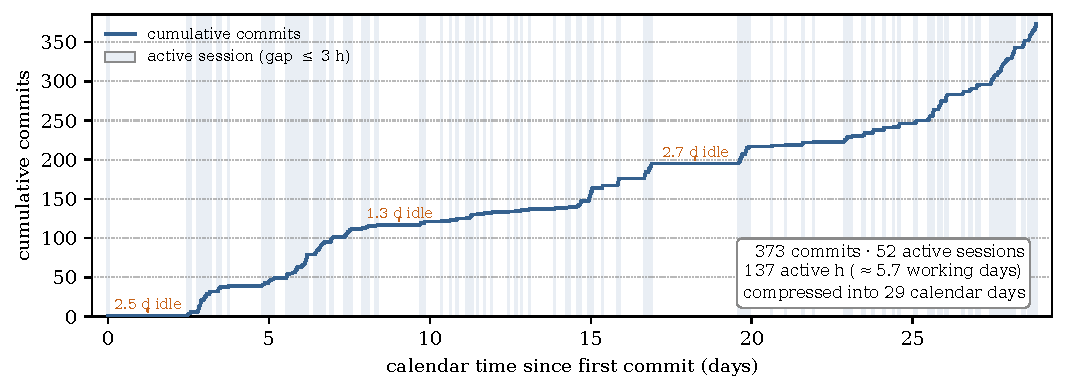
\includegraphics[width=0.98\columnwidth]{figures/fig_timeline.pdf}
\caption{Implementation effort from the version-control log. Cumulative commits
against calendar time; shaded bands are active sessions (consecutive commits no
more than three hours apart). The long flat stretches are idle gaps. The 373
commits cluster into 52 active sessions totalling ${\sim}137$ hours of
work---about 5.7 working days---spread across a 29-day calendar window.}
\label{fig:timeline}
\end{figure}

Figure~\ref{fig:timeline} visualises the effort estimate reported in the main
paper: 373 commits over a 29-day calendar span, of which the active sessions
sum to about 137 hours.

\end{document}
